
\section{Overview of Engineering
Task}\label{overview-of-engineering-task}}


\subsection{Contents}\label{contents}}


\subsection{Abstract}\label{abstract}}

Global agriculture relies heavily on herbicides use to minimize yeild
loss due to weeds, which can be significant. An issue is that no new
herbicide classes have been discovered in \href{how\%20long?}{decades},
which coupled with frequent outbreaks of herbicide resistant weeds
leaves an un-met demand for more effective weed control technology.
Engineered herbicide resistant crops are an effective solution to this
problem since they allow farmers flexibility in their herbicide
application programs, minimizing the risk of a resistance outbreak.
Their widespread adoption would also enable development of badly needed
new herbicide chemistries.

Herbicide resistance can be engineered by augmentation of the metabolic
pathways affected by the herbicide (metabolic bypassing) or by inserting
herbicide detoxification machinery. The latter can require enzyme
engineering, which is the focus of this project.

The goal of this project is to develop enzymes to initiate
detoxification of the herbicide
\href{https://pubchem.ncbi.nlm.nih.gov/compound/Mesotrione}{mesotrione},
which belongs to an important class of herbicides that inhibit 4-HPPD.

To do this, two enzyme engineering techniques are developed and
deployed.

One technique relies on virtual directed evolution - using automated
cycles of protein structure-prediction, molecular docking and mutation
by a genetic algorithm. Thousands of mutants are screened virtually and
several candidates are generated for lab testing. Lab tests on the
candidates show : \ldots{}

The other technique relies on a machine learning model that maps protein
sequence to substrate specificty, which can evaluate a large number of
sequences quickly. The model in combination with a sequence optimization
algorithm can generate candidates for lab testing. The model, trained on
in-house P450-ligand screening data can also plan subsequent rounds of
screening based on its uncertainty and the expected information gain of
a particular experiment.

\textbar\textbar\textbar{} \textbar\textbar\textbar{}
\textbar{}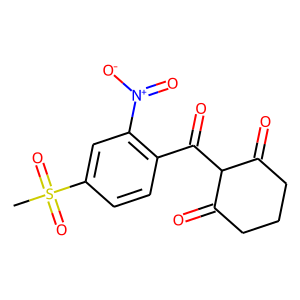
\includegraphics{pix/share/mesotrione.png}
\textbar Mesotrione, the detoxification target for this work, is a
4-HPPD inhibitor representative of the triketone class of HPPD
inhibitor.\textbar{}


\subsection{Problem Context}\label{problem-context}}

Herbice detoxification in plants is typically initiated by a ring carbon
hydroxylation by a cytochrome P450 before conjugation with glutathione
by a glutathione S-transferase (GST) and sequestration into a vacuole by
an \href{really?}{ABC transporter}. GSTs can be promiscuous so it may be
sufficient to introduce an engineered cytochrome P450 capable of
mesotrione ring hydroxylation to render a crop herbicide tolerant.
Therefore the aim of the project is to engineer a cytochrome P450
capable of a non-site specific ring hydroxylation of mesotrione.

A promising template is the cytochrome P450 BM3 from \emph{Bacillus
megatarium}, which has been extensively studied, characterized and
engineered for non-natural activity. BM3 has the fastest reaction rates
of any P450 towards its presumed natural substrate, arachadionic acid,
at 17000 MS-1 because it is naturally fused to its reductase domain.
This, combined with its ease of expression, broad engineered substrate
scope and tolerance to mutations makes BM3 a suitable template for
engineering a herbicide detoxification system.

Pilot studies indicate that neither the wild-type or the promiscuous
A82F/F87V mutant have binding activity towards mesotrione.


\subsection{Resources Available}\label{resources-available}}

Candidate solutions were devised within the constraints of the resources
available. The resources included that necesseray to perform a high
throughput screen of P450 ligand binding and the compute necesseray to
build a large neural model of sequence-substrate specificty, and to run
rounds of virtual directed evolution.


\subsubsection{Screening Equipment}\label{screening-equipment}}

Screening equipment available included:

\begin{itemize}
\tightlist
\item
  \textbf{Labcyte Echo} - an acoustic liquid handling system that can
  dispense small volumes plate-to-plate with 2.5 nl precision. Various
  models exist and all can follow arbitary dispensing instructions from
  a \texttt{csv} file.
\item
  \textbf{Thermo-Fisher Multidrop} - a bulk liquid dispensing system for
  transfer of a liquid to a microplate with speed and precision.
\item
  \textbf{BMG FluoStar Plate Readers} - micro plate readers that can
  measure the UV/visibile light absorbance between 300 and 800 nm in
  transparent plates.
\end{itemize}


\subsubsection{Compute}\label{compute}}

\begin{itemize}
\tightlist
\item
  \textbf{CPUs}
\item
  \textbf{GPUs}
\end{itemize}


\subsection{Proposed Solutions}\label{proposed-solutions}}

Two techniques are developed and field tested in this work. One is
computer program (reffered to here as \texttt{evo}) which simulates
directed evolution by cycles of structure prediction ligand docking and
mutation, directed by a genetic algorithm.

The other aims to map P450 sequence to substrate specificty with a
machine learning model that directs an enzyme-ligand screening program
in the lab by active learning. Once confident in its predictions, the
model can evaluate candidate protein sequences proposed by a sequence
optimization algorithm to generate BM3 mutants for lab testing. This
approach is asigned the moniker \texttt{rio}. test test test test test
test


\section{Project Aims}\label{project-aims}}


\subsection{Contents}\label{contents-1}}

\begin{itemize}
\tightlist
\item
  \protect\hyperlink{}{}
\end{itemize}


\subsection{Aim}\label{aim}}

The aim is to design variants of the cytochrome P450 BM3 (Cyp102A1)
capable of a non site specific hydroxylation of the herbicide
mesotrione. \#\#\# Context of Engineering Problem Wild type BM3 has no
detectable activity torwards mesotrione. BM3 is well structurally
characterised and is a popular target for P450 engineering given its
ease of production and tolerance to mutations. P450-ligand binding
activity is detectable by changes to the P450's UV-visible light
profile. \#\#\# Proposed Solutions \#\#\#\# \texttt{evo} Using BM3
structures in the PDB as templates, predict structures of BM3 mutants
and dock the target ligand to the active site and score by some
criteria. Using that process as a fitness function, use a genetic
algorithm to optimize the amino acids in the active site. The pool of
\emph{fit} mutants generated this way informs codon design.
\textgreater{} Mutants care screened for mesotrione activity with LCMS
\#\#\#\# \texttt{rio} Using a high throughput P450:ligand binding assay,
screen multiple BM3 mutants against a large compoud library. That data
can be used to train a sequence ligand specificity model. That model can
be used in design of a BM3 mutant with activity towards an arbitary
compound

\textbackslash bibliography \# Herbicide Resistance Engineering


\subsection{Contents}\label{contents-2}}

\begin{itemize}
\tightlist
\item
  \textbf{Weed Control \& Global Agriculture}
\item
  \textbf{Herbicides \& Crop Yields}
\item
  \textbf{Herbicide Resistant Weeds}
\item
  \textbf{Rate of Herbicide Development}
\item
  \textbf{Herbicide Resistant Crops}
\item
  \textbf{Herbice Resistance Engineering}
\end{itemize}

\begin{center}\rule{0.5\linewidth}{0.5pt}\end{center}


\subsection{Weed Control \& Global
Agriculture}\label{weed-control-global-agriculture}}


\subsubsection{Herbicides \& Crop Yields}\label{herbicides-crop-yields}}


\subsubsection{Herbicide Resistant
Weeds}\label{herbicide-resistant-weeds}}


\subsubsection{Rate of Herbicide
Development}\label{rate-of-herbicide-development}}


\subsubsection{Herbicide Resistant
Crops}\label{herbicide-resistant-crops}}


\subsubsection{Herbice Resistance
Engineering}\label{herbice-resistance-engineering}}


\section{Mesotrione}\label{mesotrione}}


\subsection{Contents}\label{contents-3}}

\begin{itemize}
\item
  \textbf{Herbicide Classes}
\item
  \textbf{The Herbicide Discovery Problem}
\item
  \textbf{4-Hydroxyphenyl-Pyruvate Dioxygenase (HPPD) Inhibition and
  Mechanism of Action}
\item
  \textbf{HPPD Inhibitor Development and Classes}
\item
  \textbf{HPPD Tolerance in Crops}
\item
  \textbf{HPPD Tolerance in Weeds}
\item
  \textbf{HPPD Tolerance in Weeds}
\item ~
  
  \subsection{\texorpdfstring{\textbf{Engineered HPPD-Resistance
  Crops}}{Engineered HPPD-Resistance Crops}}\label{engineered-hppd-resistance-crops}}
\end{itemize}

\begin{figure}
\centering
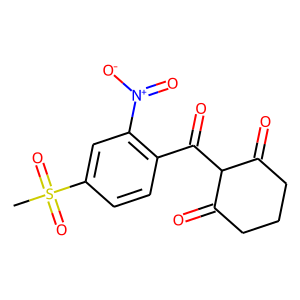
\includegraphics{pix/share/mesotrione.png}
\caption{Placeholder}
\end{figure}


\subsection{Herbicide Classes}\label{herbicide-classes}}


\subsection{The Herbicide Discovery
Problem}\label{the-herbicide-discovery-problem}}


\subsection{4-Hydroxyphenyl-Pyruvate Dioxygenase (HPPD) Inhibition and
Mechanism of
Action}\label{hydroxyphenyl-pyruvate-dioxygenase-hppd-inhibition-and-mechanism-of-action}}


\subsection{HPPD Inhibitor Development and
Classes}\label{hppd-inhibitor-development-and-classes}}


\subsection{HPPD Tolerance in Crops}\label{hppd-tolerance-in-crops}}


\subsection{HPPD Tolerance in Weeds}\label{hppd-tolerance-in-weeds}}


\subsection{HPPD Tolerance in Weeds}\label{hppd-tolerance-in-weeds-1}}


\subsection{Engineered HPPD-Resistance
Crops}\label{engineered-hppd-resistance-crops-1}}


\section{P450s}\label{p450s}}


\subsection{Contents}\label{contents-4}}

\begin{itemize}
\tightlist
\item
  \textbf{Overview}

  \begin{itemize}
  \tightlist
  \item
    \textbf{Definition}
  \item
    \textbf{Database References}
  \item
    \textbf{Common Features}
  \item
    \textbf{Common Functionality}
  \end{itemize}
\item
  \textbf{Biological Roles}

  \begin{itemize}
  \tightlist
  \item
    \textbf{Oxidoreduction}
  \item
    \textbf{Core pathways}
  \item
    \textbf{Xenobiotic metabolism}
  \end{itemize}
\item
  \textbf{Phylogenetics}

  \begin{itemize}
  \tightlist
  \item
    \textbf{Classes and Trees}
  \item
    \textbf{Conserved Motifs}
  \item
    \textbf{Mechanistic Insights}
  \end{itemize}
\item
  \textbf{Structure}

  \begin{itemize}
  \tightlist
  \item
    \textbf{Conserved Folds}
  \item
    \textbf{Heme Binding Site}
  \item
    \textbf{Ligand Binding Site}
  \end{itemize}
\item
  \textbf{Biochemical Mechanism of Action}

  \begin{itemize}
  \tightlist
  \item
    \textbf{Type I}

    \begin{itemize}
    \tightlist
    \item
      \textbf{Reaction Cycle}
    \end{itemize}
  \item
    \textbf{Type II}

    \begin{itemize}
    \tightlist
    \item
      \textbf{Reaction Cycle}
    \end{itemize}
  \item
    \textbf{Peroxidase shunt}

    \begin{itemize}
    \tightlist
    \item
      \textbf{Reaction Cycle}
    \end{itemize}
  \end{itemize}
\item
  \textbf{Experimental Techniques}

  \begin{itemize}
  \tightlist
  \item
    \textbf{UV-Vis}

    \begin{itemize}
    \tightlist
    \item
      \textbf{Soret Peak Shifts}
    \item
      \textbf{NADPH Consumption}
    \end{itemize}
  \item
    \textbf{Mass Spectrometry}
  \item
    \textbf{Crystallography}
  \item
    \textbf{NMR}
  \end{itemize}
\item
  \textbf{Applications in Biotechnology}

  \begin{itemize}
  \tightlist
  \item
    \textbf{Pharmaceutical metabolite production}
  \item
    \textbf{Agrochemical metabolite production}
  \item
    \textbf{Industrial Chemistry}
  \end{itemize}
\end{itemize}

\begin{center}\rule{0.5\linewidth}{0.5pt}\end{center}


\subsection{Overview}\label{overview}}

\begin{itemize}
\tightlist
\item
  \textbf{Definition}
\item
  \textbf{Database References}
\item
  \textbf{Common Features}
\item
  \textbf{Common Functionality} \#\# Biological Roles
\item
  \textbf{Oxidoreduction}
\item
  \textbf{Core pathways}
\item
  \textbf{Xenobiotic metabolism} \#\# Phylogenetics
\item
  \textbf{Classes and Trees}
\item
  \textbf{Conserved Motifs}
\item
  \textbf{Mechanistic Insights} \#\# Structure
\item
  \textbf{Conserved Folds}
\item
  \textbf{Heme Binding Site}
\item
  \textbf{Ligand Binding Site} \#\# Biochemical Mechanism of Action
\item
  \textbf{Type I}

  \begin{itemize}
  \tightlist
  \item
    \textbf{Reaction Cycle}
  \end{itemize}
\item
  \textbf{Type II}

  \begin{itemize}
  \tightlist
  \item
    \textbf{Reaction Cycle}
  \end{itemize}
\item
  \textbf{Peroxidase shunt}

  \begin{itemize}
  \tightlist
  \item
    \textbf{Reaction Cycle} \#\# Experimental Techniques
  \end{itemize}
\item
  \textbf{UV-Vis}

  \begin{itemize}
  \tightlist
  \item
    \textbf{Soret Peak Shifts}
  \item
    \textbf{NADPH Consumption}
  \end{itemize}
\item
  \textbf{Mass Spectrometry}
\item
  \textbf{Crystallography}
\item
  \textbf{NMR} \#\# Applications in Biotechnology
\item
  \textbf{Pharmaceutical metabolite production}
\item
  \textbf{Agrochemical metabolite production}
\item
  \textbf{Industrial Chemistry} \# BM3
\end{itemize}


\subsection{Contents}\label{contents-5}}

\begin{itemize}
\item
  \textbf{Overview}
\item
  \textbf{Short History of BM3}

  \begin{itemize}
  \tightlist
  \item
    \textbf{Host Organism and isolation}
  \item
    \textbf{Mechainism of Action Discovery}
  \item
    \textbf{Biological Role}
  \item
    \textbf{Fused Reductase and reaction speed}
  \item
    \textbf{Structure Determination}
  \item
    \textbf{Use as a Model System}
  \item
    \textbf{Use in Engineering}
  \end{itemize}
\item
  \textbf{Phylogenetics}

  \begin{itemize}
  \tightlist
  \item
    \textbf{Notable Relatives}
  \item
    \textbf{Sequence Annotation}
  \item
    \textbf{Mutation Entropy}
  \end{itemize}
\item
  \textbf{Structure}

  \begin{itemize}
  \tightlist
  \item
    \textbf{Structures Available}
  \item
    \textbf{Active site structure}
  \item
    \textbf{Ligand binding dynamics}
  \item
    \textbf{Backbone variation between mutants}
  \end{itemize}
\item ~
  
  \subsection{\texorpdfstring{\textbf{Engineering Case
  Studies}}{Engineering Case Studies}}\label{engineering-case-studies}}
\end{itemize}


\subsection{Overview}\label{overview-1}}

The bacterial cytochrome P450 BM3 will be the template enzyme for this
engineering project. It was chosen because it has been extensively
characterised, is practical to express and purify and has been the
subject of engineering efforts to alter its substrate specificity to
compounds with similar properties to some herbicides.

Wild-type \href{https://www.uniprot.org/uniprot/P14779}{cytochrome P450
BM3} (Cyp102A1, Uniprotkb: \texttt{P14779}) is a bacterial P450 found in
\emph{Bacillus megatarium} that contains a fused NADPH-P450 reductase
domain. The natural substrate is unknown, but likely to be a fatty acid
with chains of 12-16 carbons. It typically hydroxylates carbons at the
apolar tail of the chain at the omega -1,-2 and -3 positions.

The fused NADPH/P450 reductase domain is an uncharacteristic feature of
a P450, but results in a rate of reaction faster than any other known
P450 towards its preferred substrates - 17000 MS-1 in the case of
\href{https://pubchem.ncbi.nlm.nih.gov/compound/Arachidonic-acid}{arachidonic
acid} - a poly-unsaturated fatty acid with 20 carbon chain.


\subsection{Short History of BM3}\label{short-history-of-bm3}}

\begin{itemize}
\tightlist
\item
  \textbf{Host Organism and isolation}
\item
  \textbf{Mechainism of Action Discovery}
\item
  \textbf{Biological Role}
\item
  \textbf{Fused Reductase and reaction speed}
\item
  \textbf{Structure Determination}
\item
  \textbf{Use as a Model System}
\item
  \textbf{Use in Engineering} \#\# Phylogenetics
\item
  \textbf{Notable Relatives}
\item
  \textbf{Sequence Annotation}
\item
  \textbf{Mutation Entropy} \#\# Structure
\item
  \textbf{Structures Available}
\item
  \textbf{Active site structure}
\item
  \textbf{Ligand binding dynamics}
\item
  \textbf{Backbone variation between mutants} \#\# Engineering Case
  Studies
\end{itemize}


\section{Enzyme Engineering}\label{enzyme-engineering}}


\subsection{Contents}\label{contents-6}}

\begin{itemize}
\tightlist
\item
  \textbf{Overview}
\item
  \textbf{Value of Engineered Enzymes}

  \begin{itemize}
  \tightlist
  \item
    \textbf{Chemical Industry}
  \item
    \textbf{Pharmaceutical Industry}
  \item
    \textbf{Agrochemical Industry}
  \end{itemize}
\item
  \textbf{Challenges}

  \begin{itemize}
  \tightlist
  \item
    \textbf{Expensive iterations}
  \item
    \textbf{Problem Space Size}
  \item
    \textbf{Assay End Points}
  \end{itemize}
\item
  \textbf{Enzyme Engineering Techniques}

  \begin{itemize}
  \tightlist
  \item
    \textbf{Directed Evolution}
  \item
    \textbf{Computer Aided Design}

    \begin{itemize}
    \tightlist
    \item
      \textbf{Simulation-Based}

      \begin{itemize}
      \tightlist
      \item
        \textbf{\href{protein-structure-mred.md}{Structure Prediction}}
      \item
        \textbf{\href{docking.md}{Docking}}
      \item
        \textbf{\href{molecular-dynamics.md}{Molecular Dynamics}}
      \item
        \textbf{Sequence Search Algorithms}

        \begin{itemize}
        \tightlist
        \item
          Genetic Algorithms
        \item
          Bayesian Optimization
        \item
          Reinforcement Learning
        \end{itemize}
      \end{itemize}
    \end{itemize}
  \end{itemize}
\item
  \textbf{Machine Learning}

  \begin{itemize}
  \tightlist
  \item
    \textbf{Sequence-Function Mapping}

    \begin{itemize}
    \tightlist
    \item
      \textbf{Use case:} Fox et al.
    \end{itemize}
  \item
    \textbf{Pre-Trained Unsupervised Models}

    \begin{itemize}
    \tightlist
    \item
      \textbf{\texttt{esm} - facebook's transformers trained on uniprot}
      {[}@rives2021biological{]}
    \item
      \textbf{Use case} - Biswas et al.~{[}@biswas2021low{]}
    \end{itemize}
  \end{itemize}
\end{itemize}

\begin{center}\rule{0.5\linewidth}{0.5pt}\end{center}


\subsection{Overview}\label{overview-2}}


\subsubsection{Value of Engineered
Enzymes}\label{value-of-engineered-enzymes}}

\begin{itemize}
\tightlist
\item
  \textbf{Chemical Industry}
\item
  \textbf{Pharmaceutical Industry}
\item
  \textbf{Agrochemical Industry} \#\#\# Challenges
\item
  \textbf{Expensive iterations}
\item
  \textbf{Problem Space Size}
\item
  \textbf{Assay End Points} \#\# Enzyme Engineering Techniques \#\#\#
  Directed Evolution \#\#\# Computer Aided Design
\item
  De novo \& template-based {[}{]}{[}{]} \#\#\#\# Simulation-Based
  \#\#\#\#\# \href{protein-structure-mred.md}{Structure Prediction}
  \#\#\#\#\# \href{docking.md}{Docking} \#\#\#\#\#
  \href{molecular-dynamics.md}{Molecular Dynamics} \#\#\#\#\# Sequence
  Search Algorithms
\item
  Genetic Algorithms
\item
  Bayesian Optimization
\item
  Reinforcement Learning \#\#\#\# Machine Learning \#\#\#\#\#
  Sequence-Function Mapping
\item
  Fox et al. \#\#\#\#\# Pre-Trained Unsupervised Models
\item
  \textbf{\texttt{esm} - facebook's transformers trained on uniprot} -
  ESM Rives et al.
\item
  \textbf{Use case} - Biswas et al.~{[}\^{}biswas{]}
\end{itemize}

\bib


\section{General Methods}\label{general-methods}}


\subsection{Contents}\label{contents-7}}

\begin{itemize}
\item
  \textbf{Tranformation}
\item
  \textbf{DNA Purification}
\item
  \textbf{Mutation}
\item
  \textbf{Protein Expression}
\item
  \textbf{Protein Purification}
\item
  \textbf{Titration}
\item ~
  
  \subsection{\texorpdfstring{\textbf{Steady State
  Kinetics}}{Steady State Kinetics}}\label{steady-state-kinetics}}
\end{itemize}


\subsection{Tranformation}\label{tranformation}}


\subsection{DNA Purification}\label{dna-purification}}


\subsection{Mutation}\label{mutation}}


\subsection{Protein Expression}\label{protein-expression}}


\subsection{Protein Purification}\label{protein-purification}}


\subsection{Titration}\label{titration}}


\subsection{Steady State Kinetics}\label{steady-state-kinetics-1}}


\section{Introduction}\label{introduction}}


\subsection{Contents}\label{contents-8}}

\begin{itemize}
\tightlist
\item
  \textbf{Abstract}
\item
  \textbf{Background}

  \begin{itemize}
  \tightlist
  \item
    \textbf{\href{herbicide-resistance.md}{Engineering Herbicide
    Resistance}}
  \item
    \textbf{In-Silico Protein Engineering}
  \item
    \textbf{\href{protein-structure-pred.md}{Protein Structure
    Prediction}}
  \item
    \textbf{\href{docking.md}{Ligand Docking}}
  \item
    \textbf{Sequence Optimization}
  \end{itemize}
\item
  \textbf{Aim}
\item
  \textbf{Proposed Approach}
\end{itemize}

\begin{center}\rule{0.5\linewidth}{0.5pt}\end{center}


\subsection{Abstract}\label{abstract-1}}

Crop resistance to herbicides is an important tool in establishing
global food security. Herbicide resistance can be engineered into crops
by introducing an enzyme that can metaboloicly deactivate a particular
herbicide. In this work, a mutant variant of the bacterial P450 BM3
(CYP102A1) is engineered to hydroxylate the herbicide mesotrione at ring
carbon 5 as a means of deactivation. To engineer the enzyme, a virtual
directed evolution program relying on protein structure prediction,
docking and genetic algorithms is developed and deployed at scale to
adjust the BM3 active site to accomodate mesotrione in a favourable
configuration. The mutants produced by the algorithm are synthesized in
the lab and tested for expected activity.


\subsection{Background}\label{background}}


\subsubsection{\texorpdfstring{\href{herbicide-resistance.md}{Engineering
Herbicide
Resistance}}{Engineering Herbicide Resistance}}\label{engineering-herbicide-resistance}}


\subsubsection{\texorpdfstring{\emph{In-Silico} Protein
Engineering}{In-Silico Protein Engineering}}\label{in-silico-protein-engineering}}


\subsubsection{\texorpdfstring{\href{protein-structure-pred.md}{Protein
Structure
Prediction}}{Protein Structure Prediction}}\label{protein-structure-prediction}}


\subsubsection{\texorpdfstring{\href{docking.md}{Ligand
Docking}}{Ligand Docking}}\label{ligand-docking}}


\subsubsection{Sequence Optimization}\label{sequence-optimization}}


\subsection{Aim}\label{aim-1}}


\subsection{Approach}\label{approach}}


\section{Docking}\label{docking}}


\subsection{Contents}\label{contents-9}}

\begin{itemize}
\item
  \textbf{Overview}
\item
  \textbf{Applications}
\item
  \textbf{Methods \& Programs}
\item
  \textbf{Geometric}
\item
  \textbf{Autodock VINA}
\item
  \textbf{Autodock GPU}
\item ~
  
  \subsection{\texorpdfstring{\textbf{Transformers}}{Transformers}}\label{transformers}}
\end{itemize}


\subsection{Overview}\label{overview-3}}


\subsection{Applications}\label{applications}}


\subsection{Methods \& Programs}\label{methods-programs}}


\subsubsection{Geometric}\label{geometric}}


\subsubsection{Autodock VINA}\label{autodock-vina}}


\subsubsection{Autodock GPU}\label{autodock-gpu}}


\subsubsection{Transformers}\label{transformers-1}}


\section{Protein Structure
Prediction}\label{protein-structure-prediction-1}}


\subsection{Contents}\label{contents-10}}

\begin{itemize}
\tightlist
\item
  \textbf{Overview and Applications}
\item
  \textbf{Timeline of Technology Maturation}
\item
  \textbf{Physics-based Methods}
\item
  \textbf{Neural Methods}
\item
  \textbf{State of the Art and Outlook}
\end{itemize}

\begin{center}\rule{0.5\linewidth}{0.5pt}\end{center}


\subsection{Overview and Applications}\label{overview-and-applications}}


\subsection{Timeline of Technology
Maturation}\label{timeline-of-technology-maturation}}


\subsection{Physics-based Methods}\label{physics-based-methods}}


\subsection{Neural Methods}\label{neural-methods}}


\subsection{State of the Art and
Outlook}\label{state-of-the-art-and-outlook}}

{[}@rosettadock{]}

\bib


\section{Molecular Dynamics}\label{molecular-dynamics}}


\subsection{Contents}\label{contents-11}}

\begin{itemize}
\tightlist
\item
  \textbf{Overview}

  \begin{itemize}
  \tightlist
  \item
    \textbf{Purpose:} - provide a detailed model of protein dynamics and
    ligand interaction
  \end{itemize}
\item
  \textbf{Applications}

  \begin{itemize}
  \tightlist
  \item
    \textbf{Protein Dynamics}
  \item
    \textbf{Ligand Interactions}
  \end{itemize}
\item
  \textbf{Methods}
\item
  \textbf{Analysis}

  \begin{itemize}
  \tightlist
  \item
    \textbf{Visualization}
  \item
    \textbf{Dimensionality Reduction}
  \item
    \textbf{Contact Analysis}
  \end{itemize}
\item
  \textbf{Limitations}

  \begin{itemize}
  \item
    \textbf{Time scale range}
  \item
    \textbf{Computational complexity}
  \item ~
    
    \subsection{\texorpdfstring{\textbf{Computational resources and
    throughput}}{Computational resources and throughput}}\label{computational-resources-and-throughput}}
  \end{itemize}
\end{itemize}


\subsection{Overview}\label{overview-4}}

\begin{itemize}
\tightlist
\item
  \textbf{Purpose:} - provide a detailed model of protein dynamics and
  ligand interaction \#\# Applications
\item
  \textbf{Protein Dynamics}
\item
  \textbf{Ligand Interactions} \#\# Methods \#\# Analysis
\item
  \textbf{Visualization}
\item
  \textbf{Dimensionality Reduction}
\item
  \textbf{Contact Analysis} \#\# Limitations
\item
  \textbf{Time scale range}
\item
  \textbf{Computational complexity}
\item
  \textbf{Computational resources and throughput} \# Outline
\end{itemize}


\subsection{Contents}\label{contents-12}}

\begin{itemize}
\item
  \textbf{Overview}
\item
  \textbf{Protein Structure Prediction Approach}
\item
  \textbf{Ligand Docking Approach}
\item
  \textbf{Sequence Optimization}
\item
  \textbf{Mutant Design}
\item ~
  
  \subsection{\texorpdfstring{\textbf{Lab
  Testing}}{Lab Testing}}\label{lab-testing}}

  
  \subsection{Overview}\label{overview-5}}

  In order to engineer a mutant of the P450 BM3 capable of
  5-hydroxylation of the herbicide mesotrione, a virtual directed
  evoltion program was built and deployed. The program consists of a
  Darwinian genetic algorithm that iteratively generates a pool of BM3
  mutant sequences, predicts their structure based on an experimentally
  determined structure and evaluates their binding efficacy towards
  mesotrion by molecular docking. In each iteration, the \(n\) fittest
  mutants are used to generate the next mutant pool. Over several
  generations BM3 mutants with improved predicted mesotrione binding
  properties are generated, which are maded and tested for predicted
  activity in the lab.
\end{itemize}


\subsection{Protein Structure Prediction
Approach}\label{protein-structure-prediction-approach}}


\subsection{Ligand Docking Approach}\label{ligand-docking-approach}}


\subsection{Sequence Optimization}\label{sequence-optimization-1}}

\begin{Shaded}
\begin{Highlighting}[]
\CommentTok{\# psuedocode}
\KeywordTok{def}\NormalTok{ evaluate\_mutant(mutant):}
\NormalTok{    ...}

\NormalTok{population\_size }\OperatorTok{=}\NormalTok{ ... }
\NormalTok{wild\_type }\OperatorTok{=} \StringTok{\textquotesingle{}MTIKEM...\textquotesingle{}}
\NormalTok{mutant\_pool }\OperatorTok{=}\NormalTok{ [random\_point\_mutation(wild\_type) }\ControlFlowTok{for}\NormalTok{ \_ }\KeywordTok{in}\NormalTok{ population\_size]}
\ControlFlowTok{for}\NormalTok{ \_ }\KeywordTok{in} \BuiltInTok{range}\NormalTok{(n\_generations):}
\NormalTok{    scores }\OperatorTok{=} \BuiltInTok{map}\NormalTok{(evaluate\_mutant, mutant\_pool)}
\NormalTok{    best\_mutants }\OperatorTok{=}\NormalTok{ n\_best(scores, n)}
\end{Highlighting}
\end{Shaded}


\subsection{Mutant Design}\label{mutant-design}}


\subsection{Lab Testing}\label{lab-testing-1}}


\section{Methods}\label{methods}}

\begin{itemize}
\tightlist
\item
  \protect\hyperlink{overview}{\textbf{Overview}}
\item
  \protect\hyperlink{vde}{\textbf{Virtual Directed Evolution }}

  \begin{itemize}
  \tightlist
  \item
    \protect\hyperlink{sfxn}{\textbf{Fitness Function }}
  \item
    \protect\hyperlink{run}{\textbf{Run Time }}
  \end{itemize}
\item
  \protect\hyperlink{k8}{\textbf{Scaling to Cloud Infrastructure }}
\item
  \protect\hyperlink{enz}{\textbf{enz }}
\item
  \protect\hyperlink{ga}{\textbf{ga }}
\item
  \protect\hyperlink{codons}{\textbf{Codon Design }}

  \begin{itemize}
  \tightlist
  \item
    \protect\hyperlink{mxn}{\textbf{mxn }}
  \end{itemize}
\item
  \protect\hyperlink{lab}{\textbf{Lab Testing }}

  \begin{itemize}
  \tightlist
  \item
    \protect\hyperlink{labtech}{\textbf{Lab Techniques}}
  \item
    \protect\hyperlink{analysis}{\textbf{Data Analysis }}
  \end{itemize}
\end{itemize}

\begin{center}\rule{0.5\linewidth}{0.5pt}\end{center}

Overview

A system for \emph{in silico} enzyme design which simulates lab-based
directed enzyme evolution was devised. In the system, a genetic
algorithm optimises a pool of enzyme sequences towards a pre-defined
fitness score based on the outcome of a simulation that tests desired
target activity. The result is a large pool of enzyme mutant sequences,
their predicted structure, interaction with the target ligand and
assosciated fitness metrics, which can be used to inform downstream
nucleotide design for construction.

The simulation is based on protein structure prediction of the mutant
and estimation of substrate binding poses via molecular docking.
Simulations are scored by a pre-defined function that relates to desired
target activity, which are used by the genetic algorithm to generate a
new set of mutants in each iteration. Described in
\protect\hyperlink{vde}{Virtual Directed Evolution}.

\begin{verbatim}
graph TD
    a[Template sequence] -->|Single sequence| b[Repopulate and mutate] ; 
    b -->|mutant sequences| c[Predict structure] ; 
    c -->|structures| d[Dock ligand] ;
    d -->|poses| e[Score fitness] ; 
    e -->|sequence scores| f[Select fittest] ;
    f -->|mutant sequences| b ;
\end{verbatim}

The system is designed to run at scale on one or many machines using a
commercial cloud provider and cluster technologies such as Kubernetes
\texttt{\textbackslash{}ref}. Efforts to scale the process are
documented in \protect\hyperlink{k8}{Scaling to Cloud Infrastructure}.

In this project, the system was configured to optimize the BM3 active
site to accommodate a desirable binding interaction with mesotrione -
\texttt{\textbackslash{}ref\ figure}. The desired pose places the ring
carbon C5 of mesotrione adjacent to the active site heme iron, which was
hypothesized to displace the heme coordinated, heme distal water, and
initiate the hydroxylation reaction cycle, with carbon C5 as the
hydroxylation target. \protect\hyperlink{sfxn}{score fn}

!!! figure desired binding

The system was run for \(n\) generations with population sizes of \(m\)
over \(o\) compute nodes, and output a set of \(p\) mutants with
predicted favourable binding towards mesotrione.
\protect\hyperlink{codons}{Codon Design} shows how the mutants generated
by the algorithm were used to design codons

A small subset of the predicted mutants were constructed in the lab and
tested for desired activity using domain-specific analytical techniques.
\protect\hyperlink{lab}{Lab Testing} provides detail on the techniques
used and \protect\hyperlink{analysis}{Data Analysis} shows how the data
was analysed.

Several software tools were developed for this work:

\begin{itemize}
\tightlist
\item
  \protect\hyperlink{enz}{\texttt{enz}}: a python package that provides
  a simple interface to protein structure-prediction, molecular docking
  and scoring protein-ligand interactions, using \emph{pyrosetta}
  \texttt{\textbackslash{}ref} and \emph{autodock VINA}
  \texttt{\textbackslash{}ref} for template-based protein structure
  prediction and molecular docking respectively.
\item
  \protect\hyperlink{ga}{\texttt{ga}}: a python package for composition
  of custom genetic algorithms.
\item
  \protect\hyperlink{mxn}{\texttt{mxn}}: a python package that automates
  primer design for site-directed mutantgenesis.
\end{itemize}

Virtual Directed Evolution

\protect\hyperlink{evo}{\texttt{evo}} is the main repository for this
work. It contains the Scripts used to run the virtual directed evolution
experiments on a \emph{Linode} Kubernetes cluster. /* link evo repo*/

Data generated in the process is stored
\href{link\%20to\%20bucket}{here}.

The main function, \texttt{main.sh} was used to run the experiment. The
script provisions a machine from cloud provider \emph{Linode} and
configures it to run the enzyme design program. The enzyme design
program \texttt{bm3/main.py} executes for \(n\) generations with a
population size of \(m\). Experimental data is compressed and pushed to
a cloud bucket storage, then the machine is deleted.

The \texttt{bm3/main.py} program uses a genetic algorithm built using
\href{ga}{\texttt{ga}} to mutate sequences based on the promiscuous BM3
mutant A82F/F87V. Structures are predicted from the crystal structure
4KEY \texttt{\textbackslash{}ref} and docked with mesotrione using
\protect\hyperlink{enz}{\texttt{enz}}.

The main loop of \texttt{bm3/main.py} uses \href{ga}{\texttt{ga}} to
initialise a mutant population of \(n\) with random single mutants of
the template A82F/F87V sequence. Throughout the process, mutations are
constrained to hand selected active site residues.

!!! figure active site residues

Then, in each iteration the mutant structure is predicted and mesotrione
is docked to the active site using
\protect\hyperlink{enz}{\texttt{enz}}. Poses are scored based on
proximity of the mesotrione C5 to the heme iron and the VINA score, see
\href{sfxn}{Fitness function}. The top \(N%
\) fittest mutants repopulate the mutant pool via random crossover
between random pairs of sequences and a random point mutation.

The free paramaters \(n\) - the number of iterations and \(p\) the
population size were experimented with;

enz

ga

Fitness Function

Scaling to Cloud Infrastructure

Run Time

Codon Design

mxn

codons\_

Lab Testing

Lab Techniques

Data Analysis


\section{enz}\label{enz}}


\subsection{Contents}\label{contents-13}}

\begin{itemize}
\tightlist
\item
  \protect\hyperlink{}{Motivation}
\item
  \protect\hyperlink{}{Implementation}
\item
  \protect\hyperlink{}{API}
\item
  \protect\hyperlink{}{Benchmarking}
\end{itemize}


\section{Overview}\label{overview-6}}

\texttt{enz} is a \texttt{python} package developed for this work to
wrap both protein structure prediction and ligand docking with a simple
interface.


\section{Motivation}\label{motivation}}

The proposed virtual directed evolution method requires structure
prediction and docking \ldots{}


\section{Implementation}\label{implementation}}

Backends: - \texttt{nwalign} - for sequence alignment -
\texttt{pyrosetta} - for template-based structure prediction. Only side
chain repacking \texttt{ref} is used - \texttt{openbabel} - for
\texttt{pdbqt} file generation for \texttt{vina} - \texttt{vina} - for
docking - \texttt{pandas} \& \texttt{biopandas} - for \texttt{pdb} file
cleaning and data output


\section{API}\label{api}}

\textbf{Motivation:} simple

\textbf{Objects}

\textbf{Examples}

Test pull request \# Benchmarking


\section{mxn}\label{mxn}}


\subsection{Overview}\label{overview-7}}

\texttt{mxn} is a python package that automats primer design for
site-directed mutagenesis using either \emph{Agilent QuickChange} or
\emph{NEB Q5} mutagenesis kits. \# Results


\subsection{\#\# Contents}\label{contents-14}}


\subsection{\texorpdfstring{\texttt{enz}
Accuracy}{enz Accuracy}}\label{enz-accuracy}}


\subsection{Virtual Directed
Evolution}\label{virtual-directed-evolution}}


\subsubsection{Description of Mutants
Screened}\label{description-of-mutants-screened}}

\begin{itemize}
\tightlist
\item
  \textbf{Data Visualizations} \#\#\# Mutation Convergence \#\#\#
  Contact Analysis \#\#\# Mutant Design \#\#\# Degenerate Codon Design
  \#\#\# Site Directed Mutagenesis Design \#\# Lab Results \#\#\#
  Binding \#\#\# Turnover \#\#\# Prooduct Formation \# Methods
\end{itemize}


\subsection{Contents}\label{contents-15}}


\subsection{High Throughput Screening}\label{high-throughput-screening}}


\subsubsection{Assay Design}\label{assay-design}}

\begin{itemize}
\tightlist
\item
  UV-Vis spectroscopy theory
\item
  Development
\item
  Protocol

  \begin{itemize}
  \tightlist
  \item
    Coarse grained
  \item
    Fine grained
  \end{itemize}
\item
  Accuracy(?) \#\#\# Data Processing
\item
  Anomaly detectoion \#\# Model Design
\item
  Sequence encoding with \texttt{esm}
\item
  Chemical Representation with graph neural networks
\item
  Uniprot pre-training dataset \#\# Model Training and Evaluation \#\#
  Model-Driven Screening Design
\item
  Expected information Gain \#\# Model-Driven Enzyme Design \#
  Discussion
\end{itemize}


\subsection{Contents}\label{contents-16}}

\begin{center}\rule{0.5\linewidth}{0.5pt}\end{center}


\subsection{Efficacy of Designed
Mutants}\label{efficacy-of-designed-mutants}}


\subsection{Efficacy of Proposed
Technique}\label{efficacy-of-proposed-technique}}


\subsection{Suggested Improvements}\label{suggested-improvements}}


\section{Introduction}\label{introduction-1}}


\subsection{Contents}\label{contents-17}}

\begin{center}\rule{0.5\linewidth}{0.5pt}\end{center}


\subsection{Background}\label{background-1}}


\subsubsection{Overview}\label{overview-8}}

\begin{itemize}
\tightlist
\item
  Engineering Context: Herbicide Resistance
\item
  Target herbicide: mesotrione
\item
  Template Enzyme: P450 BM3
\item
  Approach: Screening and deep learning-based design
\end{itemize}

\begin{verbatim}
%%{init: {'theme':'base', 'themeVariables':{'darkMode':true, textColor:black}}}%%
graph LR
A[Sequence] --> B[Model]
C[Chemical] --> B
\end{verbatim}


\subsubsection{\texorpdfstring{\href{deep-learning.md}{Deep
Learning}}{Deep Learning}}\label{deep-learning}}


\subsubsection{\texorpdfstring{\href{hts.md}{High Throughput
Screening}}{High Throughput Screening}}\label{high-throughput-screening-1}}


\subsubsection{\texorpdfstring{\href{mesotrione.md}{Mesotrione}}{Mesotrione}}\label{mesotrione-1}}


\subsection{Aim}\label{aim-2}}


\subsection{Approach}\label{approach-1}}


\subsubsection{\texorpdfstring{\href{screening-fist.md}{Screening
Program}}{Screening Program}}\label{screening-program}}


\section{High Throughput Screening}\label{high-throughput-screening-2}}


\subsection{Contents}\label{contents-18}}

\begin{itemize}
\tightlist
\item
  \textbf{Definition \& Overview}
\item
  \textbf{Automation}
\item
  \textbf{Standardisation \& SBS}
\item
  \textbf{Dispensing}
\item
  \textbf{Multichannel Pipetting}
\item
  \textbf{Pipetting Robots}
\item
  \textbf{Bulk Dispensing}
\item
  \textbf{Low Volume \& Acoustic Dispensing}
\item
  \textbf{Reading}

  \begin{itemize}
  \tightlist
  \item
    \textbf{Plate Readers}
  \end{itemize}
\item
  \textbf{Plate Maneurvering}

  \begin{itemize}
  \tightlist
  \item
    \textbf{Arms}
  \item
    \textbf{Tracks}
  \item
    \textbf{Logistics Networks}
  \end{itemize}
\item
  \textbf{Data Management}

  \begin{itemize}
  \tightlist
  \item
    \textbf{Data Analysis}
  \item
    \textbf{Automated Data Analysis}
  \item
    \textbf{Python \& SciPy}
  \item
    \textbf{Machine Learning}
  \end{itemize}
\item
  \textbf{Cloud Services}

  \begin{itemize}
  \tightlist
  \item
    \textbf{APIs}
  \item
    \textbf{Strateos}
  \end{itemize}
\end{itemize}

\begin{center}\rule{0.5\linewidth}{0.5pt}\end{center}


\subsubsection{Definition \& Overview}\label{definition-overview}}


\subsubsection{Automation}\label{automation}}


\subsubsection{Standardisation \& SBS}\label{standardisation-sbs}}


\subsubsection{Dispensing}\label{dispensing}}

\begin{itemize}
\tightlist
\item
  \textbf{Multichannel Pipetting}
\item
  \textbf{Pipetting Robots}
\item
  \textbf{Bulk Dispensing}
\item
  \textbf{Low Volume \& Acoustic Dispensing} \#\#\# Reading
\item
  \textbf{Plate Readers} \#\#\# Plate Maneurvering
\item
  \textbf{Arms}
\item
  \textbf{Tracks}
\item
  \textbf{Logistics Networks} \#\#\# Data Management \#\#\# Data
  Analysis
\item
  \textbf{Automated Data Analysis}
\item
  \textbf{Python \& SciPy}
\item
  \textbf{Machine Learning} \#\#\# Cloud Services
\item
  \textbf{APIs}
\item
  \textbf{Strateos}
\end{itemize}


\section{Deep Learning}\label{deep-learning-1}}

\begin{itemize}
\tightlist
\item
  \textbf{Contents}
\item
  \textbf{Definition \& Applicability to Engineering}
\item
  \textbf{Machine Learning and Artificial Intelligence}
\item
  \textbf{Universal Models}
\item
  \textbf{Rectifiers}
\item
  \textbf{Gradient Descent}
\item
  \textbf{Backpropagation}
\item
  \textbf{Loss }
\item
  \textbf{Perceptrons}
\item
  \textbf{Deep Neural Networks}
\item
  \textbf{Transformers \& Protein Sequence Learning}
\item
  \textbf{Representation Learning}
\item
  \textbf{Graph Neural Networks and Chemical Learning}
\item
  \textbf{Recommender Systems}
\item
  \textbf{Active/Adaptive Learning \& Optimal Experiment Dsign}
\item
  \textbf{Current State of the Art}
\end{itemize}

\begin{center}\rule{0.5\linewidth}{0.5pt}\end{center}


\subsection{Definition \& Applicability to
Engineering}\label{definition-applicability-to-engineering}}


\subsection{Machine Learning and Artificial
Intelligence}\label{machine-learning-and-artificial-intelligence}}


\subsection{Universal Models}\label{universal-models}}


\subsection{Perceptrons}\label{perceptrons}}


\subsection{Deep Neural Networks}\label{deep-neural-networks}}


\subsection{Rectifiers}\label{rectifiers}}


\subsection{Gradient Descent}\label{gradient-descent}}


\subsection{Backpropagation}\label{backpropagation}}


\subsection{Loss}\label{loss}}


\subsection{Transformers \& Protein Sequence
Learning}\label{transformers-protein-sequence-learning}}


\subsection{Graph Neural Networks and Chemical
Learning}\label{graph-neural-networks-and-chemical-learning}}


\subsection{Recommender Systems}\label{recommender-systems}}


\subsection{Active/Adaptive Learning \& Optimal Experiment
Dsign}\label{activeadaptive-learning-optimal-experiment-dsign}}


\subsection{Current State of the Art}\label{current-state-of-the-art}}

\begin{longtable}[]{@{}l@{}}
\toprule
\endhead
\begin{minipage}[t]{0.09\columnwidth}\raggedright
\# Equations - \textbf{ReLU:} \(f(x) = max(0, x)\) - \textbf{Sigmoid:}
\(f(x) = {1 \over 1 + e^{-x}}\) - \textbf{quatratic:}
\(x = {-b \pm \sqrt{b^2-4ac} \over 2a}\) \# plates \# echo\strut
\end{minipage}\tabularnewline
\begin{minipage}[t]{0.09\columnwidth}\raggedright
\#\# Overview \texttt{echo} is a python package written to generate
custom instructions for \emph{Labcyte Echo} low volume liquid handling
machines. The output is a \texttt{csv} \emph{pick list} that specifies
the transfers to be made. \texttt{echo} keeps track of sample volumes,
which avoids under-dispensing due to a low volume error. \# cpd\strut
\end{minipage}\tabularnewline
\begin{minipage}[t]{0.09\columnwidth}\raggedright
\#\# Overview \texttt{cpd} is a python utility for selecting
structurally diverse screening compounds. \# Results\strut
\end{minipage}\tabularnewline
\begin{minipage}[t]{0.09\columnwidth}\raggedright
\#\# Contents - \textbf{Assay Accuracy} - \textbf{Chemical Space
Coverage} - \textbf{Initial Coarse Grained Screen} - \textbf{Initial
Fine Grained Screen} - \textbf{Model Pre-Training} - \textbf{Model
Training} - \textbf{Model-Guided Optimal Screening Design} -
\textbf{Model-Guided Enzyme Design}\strut
\end{minipage}\tabularnewline
\bottomrule
\end{longtable}


\subsection{Assay Accuracy}\label{assay-accuracy}}


\subsection{Chemical Space Coverage}\label{chemical-space-coverage}}


\subsection{Initial Coarse Grained
Screen}\label{initial-coarse-grained-screen}}


\subsection{Initial Fine Grained
Screen}\label{initial-fine-grained-screen}}


\subsection{Model Pre-Training}\label{model-pre-training}}


\subsection{Model Training}\label{model-training}}


\subsection{Model-Guided Optimal Screening
Design}\label{model-guided-optimal-screening-design}}


\subsection{Model-Guided Enzyme
Design}\label{model-guided-enzyme-design}}


\section{Outline}\label{outline}}


\subsection{Contents}\label{contents-19}}

\begin{itemize}
\item
  \textbf{Overview}
\item
  \textbf{Model Specification and Architecture}
\item
  \textbf{Screening Program}
\item
  \textbf{Pre Training}
\item
  \textbf{Training}
\item
  \textbf{Expected Information Gain and Optimal Experiment Design}
\item ~
  
  \subsection{\texorpdfstring{\textbf{Mutant
  Generation}}{Mutant Generation}}\label{mutant-generation}}

  
  \subsection{Overview}\label{overview-9}}

  This work attempts to build a machine learning model that maps protein
  sequence to substrate specificity. The model is pre-trained on a large
  enzyme:substrate binding dataset before being re-trained on
  domain-specific P450 BM3:ligand screening data. The model is used to
  optimally design subsequent screening rounds by estimating the
  expected information gain of an experiment. The model is also used to
  propose BM3 variant sequences with predicted binding activity towards
  mesotrione.
\end{itemize}


\subsection{Model Specification and
Architecture}\label{model-specification-and-architecture}}


\subsection{Screening Program}\label{screening-program-1}}


\subsection{Pre Training}\label{pre-training}}


\subsection{Expected Information Gain and Optimal Experiment
Design}\label{expected-information-gain-and-optimal-experiment-design}}


\subsection{Mutant Generation}\label{mutant-generation-1}}


\section{Screening}\label{screening}}


\subsection{Contents}\label{contents-20}}

\begin{itemize}
\tightlist
\item
  \textbf{Overview}
\item
  \textbf{Requirements}
\item
  \textbf{Assay Development}
\item
  \textbf{Protein Production}
\item
  \textbf{Compound Selection}
\item
  \textbf{Analysis Pipeline}
\item
  \textbf{Model Building}
\item
  \textbf{Adaptive Learning}
\end{itemize}

\begin{center}\rule{0.5\linewidth}{0.5pt}\end{center}


\subsection{Overview}\label{overview-10}}


\subsection{Requirements}\label{requirements}}


\subsection{Assay Development}\label{assay-development}}


\subsection{Protein Production}\label{protein-production}}


\subsection{Compound Selection}\label{compound-selection}}


\subsection{Analysis Pipeline}\label{analysis-pipeline}}


\subsection{Model Building}\label{model-building}}


\subsection{Adaptive Learning}\label{adaptive-learning}}


\section{Discussion}\label{discussion}}


\subsection{Contents}\label{contents-21}}


\section{References}\label{references}}
